\documentclass[11pt, oneside]{article} 
\usepackage{geometry}
\geometry{letterpaper} 
\usepackage{graphicx}
	
\usepackage{amssymb}
\usepackage{amsmath}
\usepackage{parskip}
\usepackage{color}
\usepackage{hyperref}

\graphicspath{{/Users/telliott/Github/number_theory/png/}}
% \begin{center} \includegraphics [scale=0.4] {gauss3.png} \end{center}

\title{Modular arithmetic}
\date{}

\begin{document}
\maketitle
\Large

\begin{center} 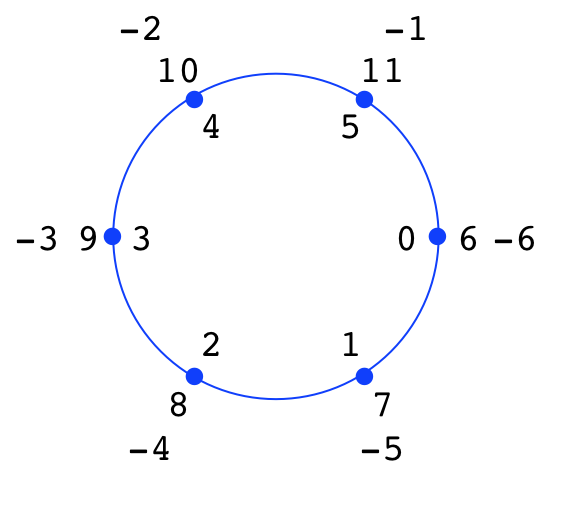
\includegraphics [scale=0.3] {clock_arithmetic.png} \end{center}

Modular arithmetic is sometimes called "clock" arithmetic.  Modular arithmetic is all of

$\circ$ \ addition

$\circ$ \ multiplication

$\circ$ \ subtraction

$\circ$ \ division

with integers, all carried out modulo (or mod) some integer $n$. The rule is to keep the remainder after dividing by the modulus.  This is the "mod" operation.

We say that $5 = 17$ mod $12$.  A new term is introduced:  congruence.  $5$ is congruent to $17$ mod $12$ and the symbol for that is $5 \equiv 17$.

Hardy:

\begin{quote}The absolute values of numbers are comparatively unimportant; we want to know what time it is, not how many minutes have passed since the creation.\end{quote}

\subsection*{Addition}

Here is an addition table for $n = 7$:

\begin{verbatim}
    0  1  2  3  4  5  6
   ---------------------
0 | 0  1  2  3  4  5  6
1 | 1  2  3  4  5  6  0
2 | 2  3  4  5  6  0  1
3 | 3  4  5  6  0  1  2
\end{verbatim}

Example:  $3 + 5 = 8 \equiv 1  \text{ mod } 7$.

Since $36  \text{ mod } 7 = 1$ and $15 \text{ mod } 7 = 1$ as well, it follows that
\[ 36 \equiv 15 \equiv 1 (\text{ mod } 7)\]

\newpage

\subsection*{Multiplication}

\begin{verbatim}
  7
  1  |  0  1  2  3  4  5  6
  2  |  0  2  4  6  1  3  5
  3  |  0  3  6  2  5  1  4
  4  |  0  4  1  5  2  6  3
  5  |  0  5  3  1  6  4  2
  6  |  0  6  5  4  3  2  1
\end{verbatim}

\begin{verbatim}
 12
  1  |  0   1   2   3   4   5   6   7   8   9  10  11
  2  |  0   2   4   6   8  10   0   2   4   6   8  10
  3  |  0   3   6   9   0   3   6   9   0   3   6   9
  4  |  0   4   8   0   4   8   0   4   8   0   4   8
  5  |  0   5  10   3   8   1   6  11   4   9   2   7
  6  |  0   6   0   6   0   6   0   6   0   6   0   6
  7  |  0   7   2   9   4  11   6   1   8   3  10   5
  8  |  0   8   4   0   8   4   0   8   4   0   8   4
  9  |  0   9   6   3   0   9   6   3   0   9   6   3
 10  |  0  10   8   6   4   2   0  10   8   6   4   2 
 11  |  0  11  10   9   8   7   6   5   4   3   2   1 
\end{verbatim}

The tables were constructed by standard multiplication, followed by the indicated mod operation.

We see certain patterns:  

$\circ$ \ For $n = 12$ factors which are co-prime to 12 (2, 3, 4, 6, 8, 9, 10) cycle back to $0$ more than once, as a consequence they cannot generate all values $< n$ as products.  The period $t$ is such that $a \cdot t \equiv 0$ mod $n$.

$\circ$ \ Also for $n=12$, rows made by multiplication of primes generate all the integers less than $12$.  

$\circ$ \ It's always true that $1$ and $n-1$ generate all the values $< n$.  

That's because
\[ a \cdot b + a \cdot (n-b) \]
\[ = ab + an - ab \]
\[ = na \equiv 0 \ (\text{ mod n }) \]

So for example, with $b=3$ we had $11 \cdot 3 = 9$ and $11 \cdot 9 = 3$, which add to zero, mod $12$.

For $n = 7$, every number generated all the other ones.  This always happens for $n$ prime.

\subsection*{important}

Since all integers smaller than n are generated from each starting integer in the special case, a \emph{unique result must be produced for each multiplication}.

Further, if a number, multiplied by all the elements of the field generates all the elements of the field, then  exactly one of those results must be equal to $1$.  

The two multiplicands with this property are called \emph{multiplicative inverses}. 

An interesting case is one where n is not prime, yet certain integers other than $1$ and $n-1$ generate all the integers smaller than $n$.  This happens when the smaller number is co-prime with $n$ (they have no common factors other than $1$).

For example, neither $10$ nor $21$ is prime but the row for times $10$ mod $21$ is:

\begin{verbatim}
10 20 9 19 8 18 7 17 6 16 5 15 4 14 3 13 2 12 1 11
\end{verbatim}

which is itself something to think about.

\subsection*{Division}

Consider multiplication mod n = 7 again:

\begin{verbatim}
  7
  1  |  0  1  2  3  4  5  6
  2  |  0  2  4  6  1  3  5
  3  |  0  3  6  2  5  1  4
  4  |  0  4  1  5  2  6  3
  5  |  0  5  3  1  6  4  2
  6  |  0  6  5  4  3  2  1
\end{verbatim}

Since $2 \cdot 4 = 1$ (mod 7), 4 and 2 are \emph{multiplicative inverses}.

Similarly $(3,5)$, $(6,6)$ and$(1,1)$ are as well.

We claim that division by $q$ is the same as multiplication by the multiplicative inverse of $q$ since, e.g.
\[  \frac{5}{4} = \frac{5}{4} \cdot \frac{2}{2} = 5 \cdot 2 \equiv 3 \ (\text{ mod } 7) \]
which can be checked by
\[ 3 \cdot 4 \equiv 5 \]

\subsection*{Powers}

With $n = 7$, consider the powers of each $ i < 7$:

\begin{verbatim}
    1  2  3  4  5  6
   ---------------------
1 | 1  2  3  4  5  6
2 | 2  4  1  2  4  1
3 | 3  2  6  4  5  1
4 | 4  2  1  4  2  1
5 | 5  4  6  2  3  1  
6 | 6  1  6  1  6  1
\end{verbatim}

This table can be a challenge to construct.  I wrote a script to help with the calculations the first time through. 

We discover that the powers of $3$ and $5$ (but not $2,4,6$) give all the integers $<7$.  

We see another interesting pattern, that each $a < n$ raised to the $n-1$ power, is equal to one.  This is explained by Fermat's little theorem, which we'll get to.

This is what wikipedia means when they talk about the "q - 1 power of unity".

\end{document}